\section{Datasets}
\label{sec:datasets}

\begin{figure*}
  \label{fig:shanghai}
  \centering
  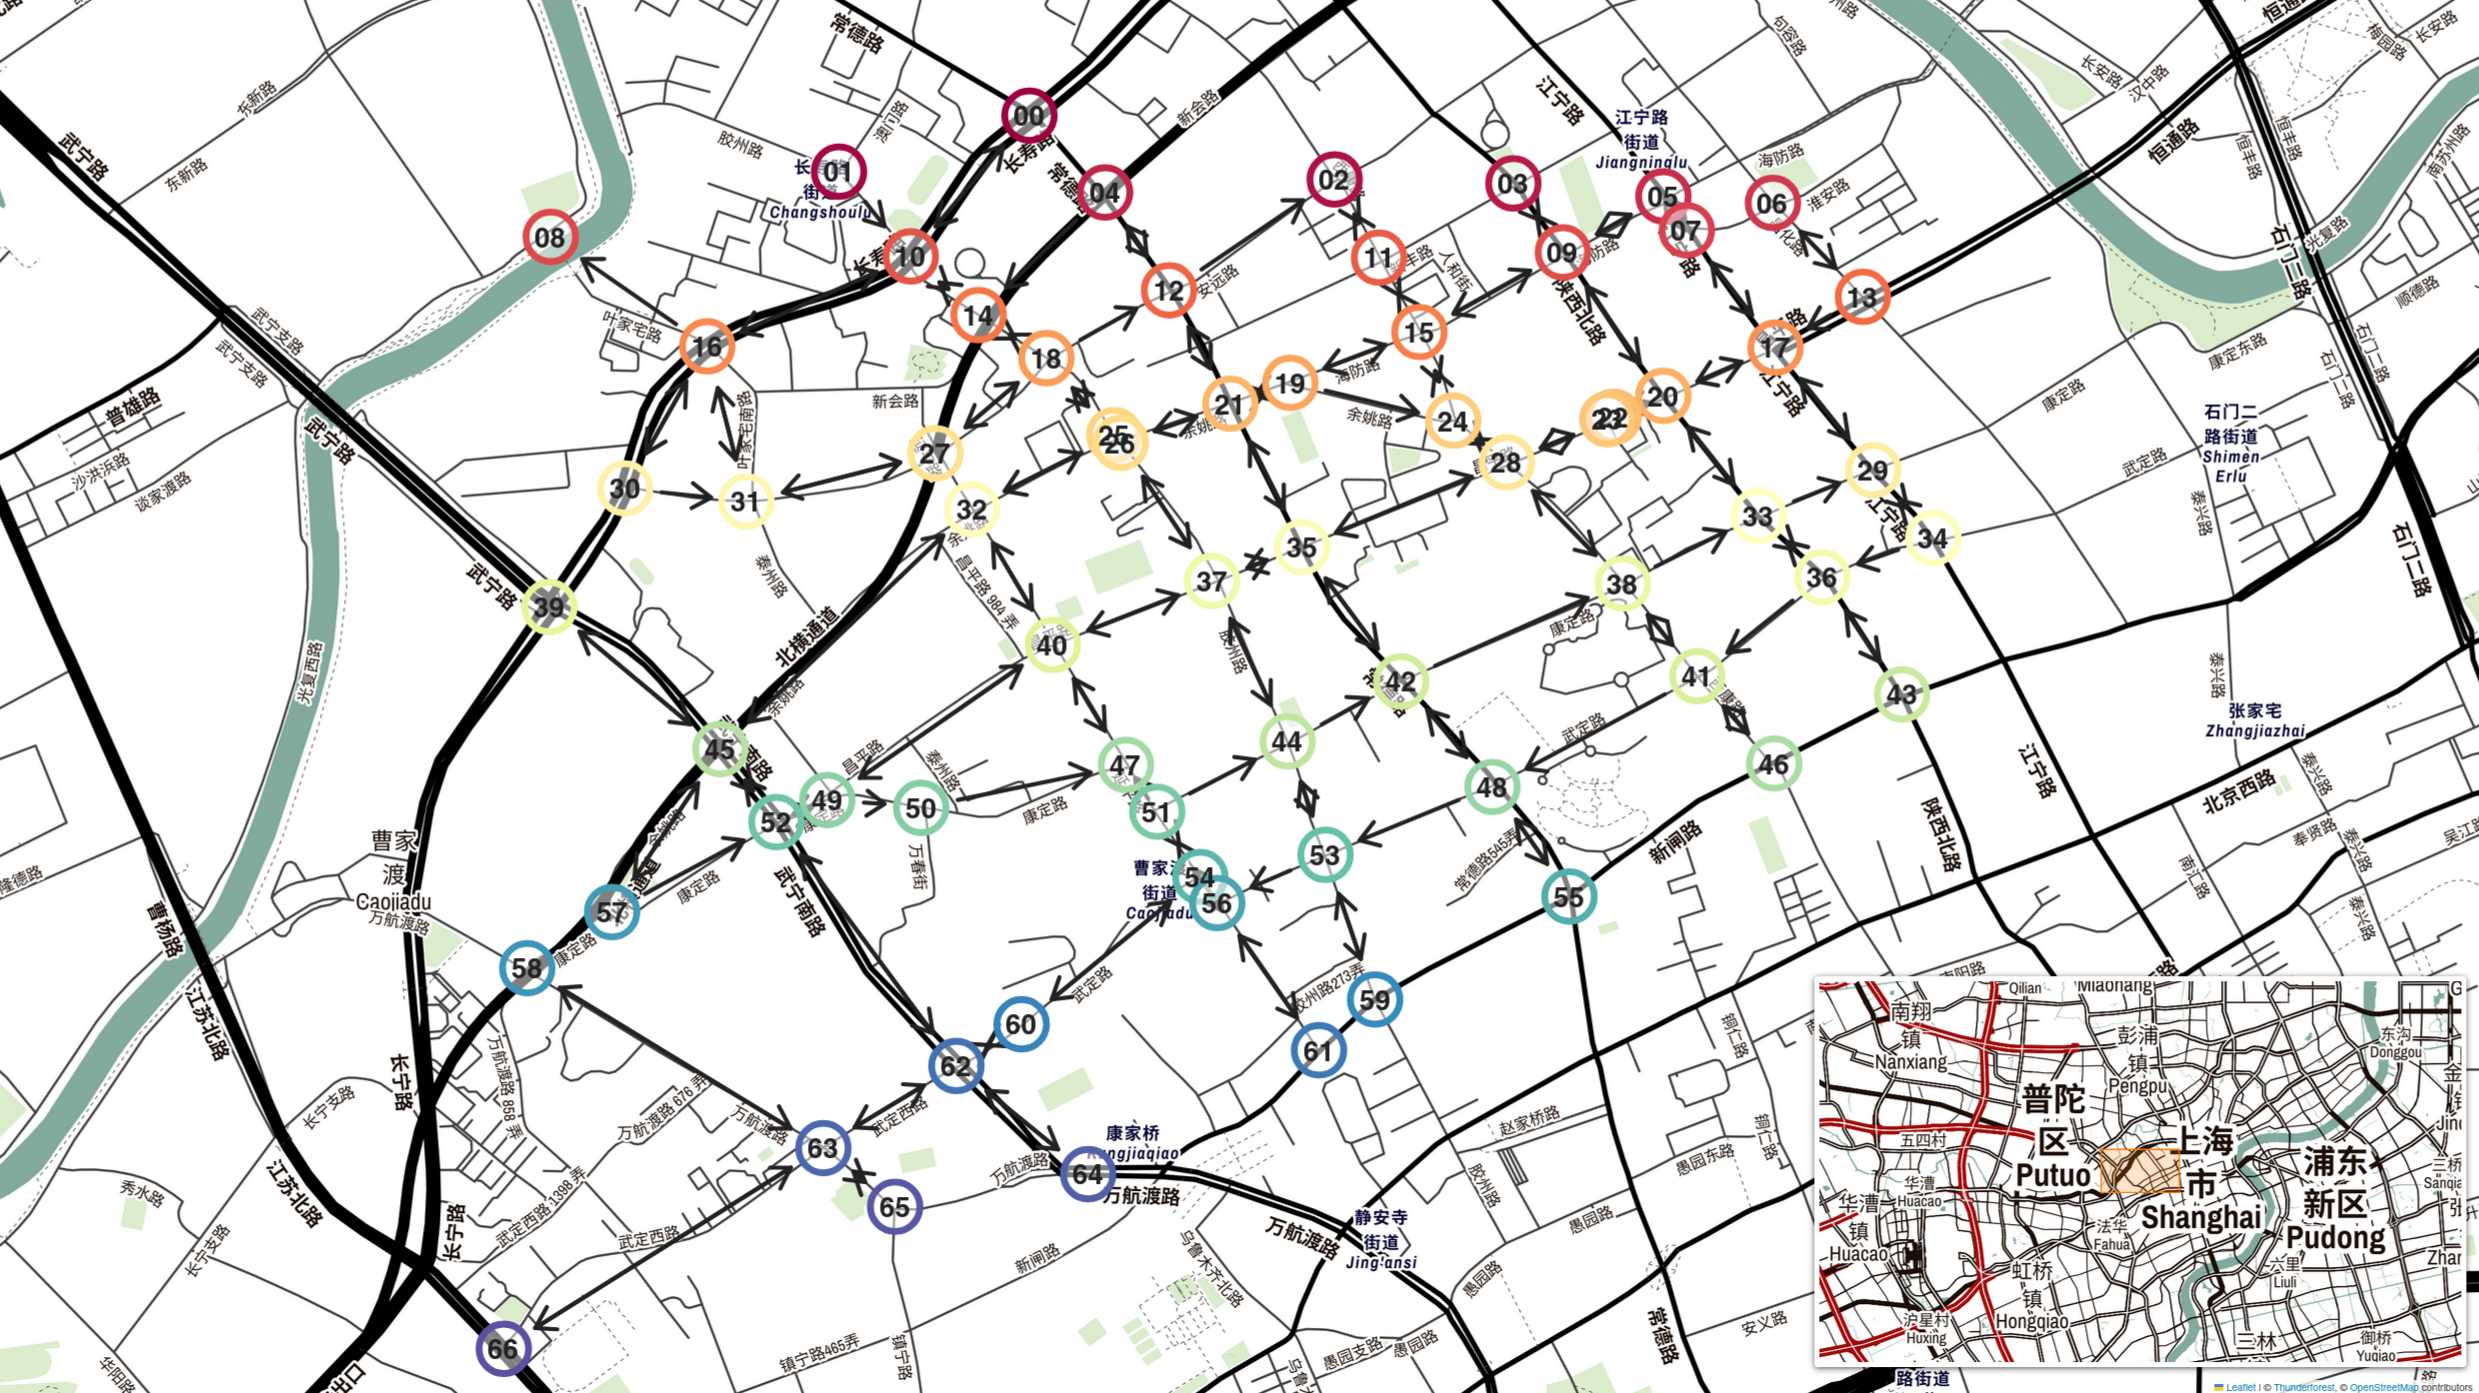
\includegraphics[width=\textwidth]{figures/06-06-2026-152435.png}
  \vspace{-5pt}
  \caption{The vertices $V$ of the dataset in Shanghai, coloured by their integer representation in order to alleviate finding particular vertices. For an interactive map visit the project's GitHub Pages on \href{https://finnharbeke.github.io/shortest-path-portfolios/shanghai.html}{finnharbeke.github.io}.}
\end{figure*}

Throughout \cref{sec:stats,sec:portfolios,sec:graphwide} we will study the \nameref{prob:shortest-path} through the lens of a specific instance. We use a real-world traffic dataset, derived from taxi trajectory data collected by the Shanghai Transportation Information Center (TIC). The data is originally introduced by \citeauthor{wangDataFusion}, using the TIC taxi trajectory data of the entire city. In the same year, \citeauthor{grnn} selected a subgraph thereof, for which there exists an entire time series, for use in metropolitan traffic prediction and made that dataset publicly accessible\footnote{\url{https://github.com/xxArbiter/grnn}}. This subgraph spans between the south-west of Jing'An district and the eastern end of Putuo. The graph does not span a very large area, spanning not more than 3 kilometers in both the north-south as well as the east-west directions. It is depicted in \cref{fig:shanghai}.

\subsection{Preprocessing}

The raw data consists of average vehicle speeds (in km/h) for each road segment, aggregated over 10-minute intervals from taxi GPS trajectories. For our purposes, we convert these speeds into travel times. Because the coordinates of every intersection is part of the data, we can compute the length of each road segment by using the haversine distance between intersections. This introduces a small source of error for road segments with bends, which seems negligable when looking at \cref{fig:shanghai} more closely. Thus, for a road segment $e$ of length $\ell_e$ (in metres) with observed speed $s_e$ (in km/h) at a given time interval, the travel time is
\[
c(e) = \frac{\ell_e}{s_e} \cdot \frac{60}{1000}.
\]
in minutes.

There are a total of $N = 4320$ 10-minute intervals where the taxi travel speeds have been recorded. This provides us with exacltly $N$ edge cost functions.
In order to get a feel for the typical speeds and the behaviour patterns of the dataset, we visualize the raw data in \cref{fig:april}.

\begin{figure*}
  \label{fig:april}
  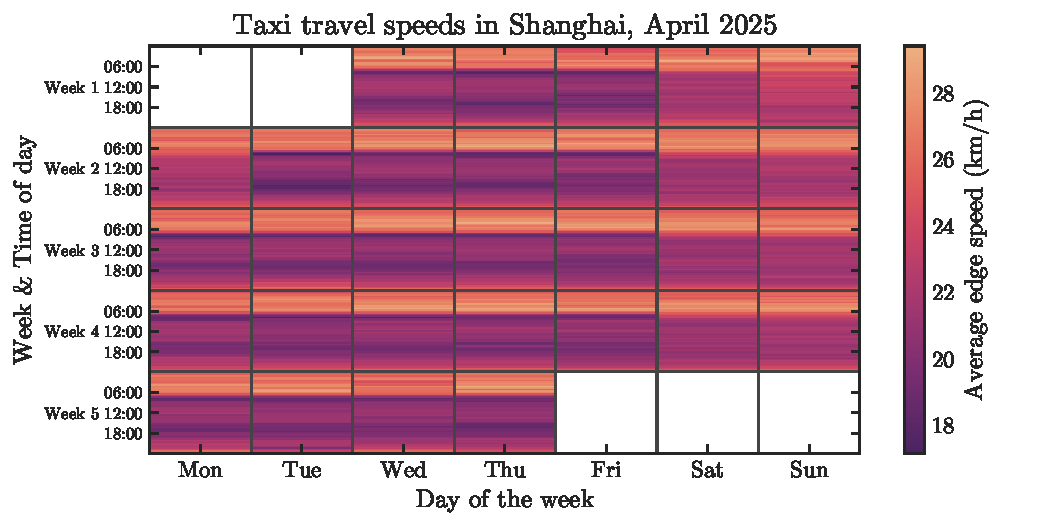
\includegraphics[width=\textwidth]{figures/apr2015.pdf}
  \caption{The graph-wide mean travel speed for every recorded 10-minute interval in the original dataset used by \cite{grnn}. The intervals span between April 1st and April 30th 2015. They are arranged in a calendar-like view in order to highlight patterns such as rush hours and the less congested weekends.}
\end{figure*}

\subsection{The Shanghai Instance}

\begin{instance}[Shanghai Taxi]
\label{shanghai}
Let $G_s = (V_s, E_s)$ be the graph from the Shanghai dataset, where $V_s$ are the intersections and $E_s$ the road segments. Let $\mathcal C_s$ be the $N_s$ edge costs reported over 10-minute intervals during April 2015 and $\mathcal D_s$ the uniform distribution over the set $\mathcal C_s$. Then $(G_s, \mathcal C_s, \mathcal D_s)$ is an instance of \cref{prob:shortest-path}.
\end{instance}

\Cref{shanghai} is a very useful problem instance to start studying the \nameref{prob:shortest-path} problem in an exploratory manner. See \cref{tab:shanghai-stats} for some statistics. With 67 vertices, $G_s$ is by no means a big graph, but it is large enough to possess distinct neighbourhoods and different road policies, such as both one-way and two-way streets. The relatively little size allows for exploring algorithms with exponential running time, that can serve as a reference, see \cref{sec:portfolios}. This is also by virtue of its sparseness, with an average vertex out-degree of less than 2.5.
On the other hand there are various sides to the dataset that make clear it will not be able to provide us with the full picture of \cref{prob:shortest-path} instances on real-life data. Since the graph is a somewhat arbitrarily cut off subgraph, there are missing edges between some of the outer vertices that would have likely provided the actual shortest paths, see vertices $43, 46, 55, \dots$ along the most south-east street in \cref{fig:shanghai}. Then there seem to be two pairs of vertices, $22,23$ and $25,26$, that are on the same intersection, but don't share any edge. This could be entirely truthful due to some obstruction on the road, but it is likely to be an error in the data.
But most importantly the average travel time between any two vertices is typically less than 5, and never more than 10 minutes (\cref{fig:shanghai_hist}). In 2019, the average commute time in Shanghai was 42 minutes\footnote{Source: \href{https://service.shanghai.gov.cn/sheninfo/specialdetail.aspx?Id=01de1f87-936d-4999-ba8c-0dffaa397ffb}{shanghai.gov.cn}}. While this might be longer than the average taxi trip, the taxi trips are likely to also take longer than 3-8 minutes. Thus, we argue that the time savings gained from analysing a graph of this size would probably only affect the last mile of many actual taxi trips. \todo[inline]{I don't understand what this statement means -- do we want to say that the gains are ? they do not necessarily come from the very last mile of the trip right?} While the last mile problem\footnote{See \href{https://en.wikipedia.org/wiki/Last\_mile\_(transportation)}{wikipedia.org}} is a well-known problem it typically refers to logistics or public transport networks, rather than taxi or car trips.

\renewcommand{\arraystretch}{1.2}
\begin{table}[htbp]
\centering
\begin{tabular}{lr}
\textbf{Property} & \textbf{Value} \\
\hline
Vertices ($n$) & 67 \\
Directed edges ($m$) & 156 \\
Edge cost unit & Travel time (minutes) \\
Interval duration & 10 minutes \\
Dataset time span & 1.-30. of April 2015 \\
Total recorded intervals ($N$) & 4320 \\
\hline
\end{tabular}
\vspace{5pt}
\caption{Summary of the Shanghai road network dataset.}
\label{tab:shanghai-stats}
\end{table}


